\documentclass[a4paper, 11pt]{report}
\usepackage{a4wide}
\usepackage[utf8]{vietnam}
\usepackage{tikz}
\usetikzlibrary{shapes.geometric, shapes.symbols, arrows.meta, positioning, fit, backgrounds, calc}
\usepackage[left=2.50cm, right=2.50cm, top=2.50cm, bottom=2.5cm]{geometry}
\usepackage{wrapfig} % Cho phép văn bản bao quanh hình ảnh
\usepackage{titlesec} % Tuỳ chỉnh định dạng tiêu đề (chapter, section, subsection)
\usepackage{graphicx} % Chèn hình ảnh vào tài liệu
\usepackage{listings} % Chèn code
\usepackage{alltt} % Hiển thị đúng định dạng theo src code
\usepackage{algorithm}
\usepackage{mdframed}
\usepackage{amsmath}
\usepackage{lipsum}
\usepackage{amssymb}
\usepackage{caption, subcaption}  
\usepackage{xcolor} % Sử dụng màu sắc trong báo cáo
\usepackage{url}
\usepackage{array}
\usepackage{titlefoot}
\usepackage[
    bookmarks,  
    hidelinks,  
    colorlinks=true,
    urlcolor=blue,
    citecolor=blue,
    linkcolor=black
]{hyperref}
\usepackage{float}
\usepackage{fancyhdr} % Tuỳ chỉnh header and footer
\usepackage{lastpage}
\usepackage{etoolbox} % Để tùy chỉnh page style sau \include
\usepackage{ocg-p}
\usepackage{amsmath}

\usepackage{booktabs} % Tạo bảng đẹp hơn
\usepackage{multirow} % Gộp ô theo hàng dọc
\usepackage{makecell} % Căn chỉnh nội dung ô bảng
\usepackage{array}    % Tùy chỉnh cột bảng
\usepackage{caption}  % Tùy chỉnh caption bảng
\newcolumntype{C}[1]{>{\centering\arraybackslash}m{#1}}
\usepackage{algorithmicx}
\usepackage{algpseudocode}

\definecolor{codegreen}{rgb}{0,0.6,0}
\definecolor{codegray}{rgb}{0.5,0.5,0.5}
\definecolor{codepurple}{rgb}{0.58,0,0.82}
\definecolor{backcolour}{rgb}{0.95,0.95,0.92}

\lstset{
    backgroundcolor=\color{backcolour},   
    commentstyle=\color{codegreen},
    keywordstyle=\color{magenta},
    numberstyle=\tiny\color{codegray},
    stringstyle=\color{codepurple},
    basicstyle=\ttfamily\footnotesize,
    breakatwhitespace=false,         
    breaklines=true,                 
    captionpos=t,                    
    keepspaces=true,                 
    numbers=left,                    
    numbersep=5pt,                  
    showspaces=false,                
    showstringspaces=false,
    showtabs=false,                  
    tabsize=4,
    frame=single,
    rulecolor=\color{black},
    aboveskip=1em,
    belowskip=1em
}
\setlength{\parindent}{0pt}

% Cấu hình fancyhdr
\pagestyle{fancy}
\fancyhf{} % Xóa tất cả các trường header và footer hiện tại

% Thiết lập header mới
\lhead{\textbf{IT4015 - Nhập môn An toàn thông tin}}
\renewcommand{\headrulewidth}{0.4pt}

\newcommand{\algorithmautorefname}{Thuật toán}
\renewcommand{\contentsname}{Mục lục}
\renewcommand{\chaptername}{Chương}
\renewcommand{\figurename}{Hình}
\renewcommand{\tablename}{Bảng}
\renewcommand{\lstlistingname}{Đoạn mã}
\setlength{\headheight}{14pt}

\setcounter{secnumdepth}{3}

\begin{document}
\begingroup
    \pagestyle{empty}
    \begin{titlepage}
    \begin{center}
        \Large\textbf{ĐẠI HỌC BÁCH KHOA HÀ NỘI}\\
        \vspace{0.5cm}
        \Large\textbf{TRƯỜNG CÔNG NGHỆ THÔNG TIN \& TRUYỀN THÔNG}\\
        
        \vspace{1.5cm}
        
\includegraphics[width=.8\textwidth]{images/hust-soict.png}

        \vfill
        
        \rule{16cm}{0.5mm}
        \Huge\textbf{Báo Cáo Nhập môn An toàn thông tin}\\
        
        \vspace{0.5cm}
        
        \Large\textbf{Đề tài: \textcolor{blue}{Các cơ chế phát hiện xâm nhập mạng}}\\
        \rule{16cm}{0.5mm}
        \vfill\vfill
        \LARGE\textbf{Học phần: \textcolor{blue}{Nhập môn An toàn thông tin}}\\
        \vspace{0.5cm}
        \Large\textbf{Mã học phần: IT4015}\\
    \end{center}
    \vfill
    \begin{center}
    \renewcommand{\arraystretch}{2.0}
        \begin{tabular}{l l l}
            \large\bf Giảng viên hướng dẫn: & \large\bf PGS. TS. Nguyễn Linh Giang\\
            \large\bf Sinh viên thực hiện: & \large\bf 
             Nguyễn Đình Tuấn Minh & \large\bf 20230048 \\
             & \large\bf 
             Vũ Đức Tâm & \large\bf 20230064 \\
             & \large\bf 
             Nguyễn Gia Khánh & \large\bf 202416803 \\
             & \large\bf 
             Nguyễn Đăng Cao Tuấn & \large\bf 202400119 \\
             
        \end{tabular}
    \end{center}
    \vfill
    \begin{center}
        \Large\textbf{Hà Nội, \today}
    \end{center}
\end{titlepage}
\endgroup

\begingroup
    \tableofcontents
    \thispagestyle{empty}
\endgroup

\pagestyle{fancy}
\chapter*{Lời nói đầu}
\addcontentsline{toc}{chapter}{Lời nói đầu} % Đưa Lời nói đầu vào mục lục

Trong kỷ nguyên số hóa, hệ thống mạng là nền tảng cho hầu hết hoạt động của tổ chức và doanh nghiệp. Cùng với lợi ích đó, các rủi ro an ninh mạng cũng xuất hiện thường xuyên hơn, đặc biệt là các hành vi thăm dò, khai thác dịch vụ và truyền dữ liệu bất thường qua những giao thức hợp lệ.

Trong bối cảnh đó, các biện pháp phòng thủ tĩnh như tường lửa vẫn cần thiết nhưng chưa đủ để quan sát nội dung và hành vi của lưu lượng mạng. Hệ thống phát hiện xâm nhập mạng (NIDS) giúp bổ sung lớp giám sát, tạo cảnh báo khi lưu lượng có dấu hiệu bất thường hoặc khớp với mẫu tấn công đã biết.

Trong khuôn khổ học phần \textbf{IT4015 - Nhập môn An toàn thông tin}, nhóm em lựa chọn thực hiện đề tài: \textbf{"Các cơ chế phát hiện xâm nhập mạng"}. Trọng tâm của bài tập lớn là xây dựng một NIDS nhỏ gọn bằng Python để minh họa quy trình thu thập gói tin, chuẩn hóa dữ liệu, phát hiện theo hành vi, phát hiện theo chữ ký và hiển thị cảnh báo.

Mục tiêu của báo cáo là trình bày ngắn gọn cơ sở lý thuyết cần thiết, mô tả kiến trúc hệ thống đã triển khai, kiểm thử trong môi trường lab và chỉ ra các giới hạn còn tồn tại.

Mặc dù đã nỗ lực tìm hiểu và tổng hợp tài liệu, song do giới hạn về mặt thời gian cũng như kinh nghiệm thực tiễn, bản báo cáo chắc chắn không tránh khỏi những thiếu sót. Nhóm em rất mong nhận được sự nhận xét và góp ý quý báu từ thầy để kiến thức của nhóm chúng em được hoàn thiện hơn.

Em xin chân thành cảm ơn!

\vspace{1.5cm} % Tạo khoảng trống trước phần chữ ký
\begin{flushright}
    \textit{Hà Nội, ngày 24 tháng 06 năm 2026} \\
    \vspace{0.2cm}
    \textbf{Nhóm sinh viên thực hiện} \\
    \vspace{0.5cm}
    \textbf{} 
\end{flushright}

\chapter{Giới thiệu đề tài}

\section{Bối cảnh và lý do chọn đề tài}
Trong các hệ thống mạng hiện đại, tường lửa chỉ là một lớp bảo vệ ban đầu. Nhiều cuộc tấn công vẫn đi qua các cổng hợp lệ như HTTP, DNS hoặc HTTPS, sau đó khai thác điểm yếu ở tầng ứng dụng hoặc tạo ra các hành vi bất thường trong mạng nội bộ. Vì vậy, hệ thống phát hiện xâm nhập mạng NIDS là một thành phần quan trọng để giám sát lưu lượng, phát hiện dấu hiệu tấn công và hỗ trợ quản trị viên phản ứng kịp thời.

Đề tài này tập trung xây dựng một hệ thống NIDS nhỏ gọn bằng ngôn ngữ Python nhằm minh họa các thành phần cốt lõi của một hệ thống phát hiện xâm nhập: thu thập gói tin, chuẩn hóa dữ liệu, phát hiện theo hành vi, phát hiện theo chữ ký, lưu trữ cảnh báo và hiển thị qua giao diện Dashboard. Mục tiêu chính là phục vụ học tập và trình diễn kỹ thuật, không hướng tới thay thế các hệ thống thương mại lớn như Suricata hoặc Zeek.

\section{Mục tiêu đề tài}
Bài tập đặt ra các mục tiêu sau:
\begin{itemize}
    \item \textbf{Thu thập và chuẩn hóa gói tin:} Đọc lưu lượng từ tệp PCAP hoặc giao diện mạng trực tiếp bằng thư viện Scapy, sau đó chuyển đổi thành cấu trúc sự kiện thống nhất.
    \item \textbf{Phát hiện theo hành vi:} Triển khai các luật dựa trên cửa sổ thời gian để nhận diện quét cổng, ICMP flood, TCP SYN flood và dấu hiệu DNS tunneling.
    \item \textbf{Phát hiện theo chữ ký và Chỉ số thỏa hiệp IOC:} Xây dựng bộ phân tích cú pháp cho một tập con cú pháp kiểu Suricata và kiểm tra các mẫu chỉ số thỏa hiệp IOC như danh sách đen tên miền hoặc truy vấn DNS đã biết.
    \item \textbf{Ghi nhận và trực quan hóa cảnh báo:} Lưu cảnh báo dưới dạng JSON Lines và hiển thị thống kê qua giao diện web Flask.
    \item \textbf{Kiểm thử trong môi trường thực nghiệm:} Mô phỏng các luồng tấn công phổ biến bằng công cụ tấn công trên hệ điều hành Kali Linux để đánh giá khả năng kích hoạt cảnh báo của hệ thống.
\end{itemize}

\section{Đối tượng và phạm vi nghiên cứu}
Đối tượng nghiên cứu là hệ thống phát hiện xâm nhập mạng dạng thụ động. Hệ thống quan sát lưu lượng, tạo cảnh báo và phục vụ phân tích, nhưng không trực tiếp chặn gói tin hoặc ngắt phiên kết nối như một hệ thống ngăn chặn xâm nhập IPS.

Phạm vi triển khai của bài tập lớn được giới hạn như sau:
\begin{itemize}
    \item Hệ thống xử lý các trường thông tin phổ biến của giao thức IP, TCP, UDP, ICMP và DNS.
    \item Phần phát hiện hành vi sử dụng ngưỡng tĩnh và cửa sổ trượt thời gian; các ngưỡng này là các giá trị lab/demo, cần hiệu chỉnh theo đặc tính của từng mạng thực tế.
    \item Phần chữ ký hỗ trợ một Suricata-style subset, đủ cho tình huống demo khớp tên miền chỉ số thỏa hiệp IOC mẫu trong truy vấn DNS.
    \item Hệ thống chưa giải mã TLS hoặc HTTPS, chưa tái tạo đầy đủ luồng dữ liệu TCP stream và chưa được tối ưu cho lưu lượng mạng tốc độ cao.
\end{itemize}

\section{Phương pháp thực hiện}
Đề tài được triển khai theo hướng kết hợp lý thuyết và thực nghiệm:
\begin{itemize}
    \item Nghiên cứu các cơ chế IDS cơ bản, đặc biệt là phát hiện theo chữ ký và phát hiện theo hành vi.
    \item Thiết kế kiến trúc dạng đường ống dẫn dữ liệu gồm các khối thu thập gói tin, bộ giải mã và phân tích cú pháp, động cơ luật phát hiện, bộ lưu trữ và giao diện hiển thị.
    \item Cài đặt từng module bằng Python, sử dụng Scapy cho xử lý gói tin và Flask cho giao diện web.
    \item Viết luật kiểm thử và kịch bản tấn công mô phỏng để kiểm tra kết quả cảnh báo.
    \item Đối chiếu kết quả với phạm vi đã đặt ra, đồng thời chỉ ra hạn chế còn tồn tại.
\end{itemize}

\section{Bố cục báo cáo}
Báo cáo gồm 5 chương:
\begin{itemize}
    \item \textbf{Chương 1: Giới thiệu đề tài} -- trình bày bối cảnh, mục tiêu, phạm vi và phương pháp thực hiện.
    \item \textbf{Chương 2: Cơ sở lý thuyết} -- tóm tắt các khái niệm IDS, NIDS, thuật toán so khớp chữ ký và phát hiện theo hành vi.
    \item \textbf{Chương 3: Kiến trúc và triển khai hệ thống} -- mô tả các module chính, cơ chế bộ giải mã chuẩn hóa dữ liệu và cách dữ liệu đi qua hệ thống.
    \item \textbf{Chương 4: Kịch bản thử nghiệm và đánh giá} -- trình bày môi trường phòng thí nghiệm, các kịch bản tấn công và phân tích cấu trúc nhật ký cảnh báo chi tiết.
    \item \textbf{Chương 5: Kết luận và hướng phát triển} -- tổng kết kết quả đạt được, hạn chế và hướng cải tiến.
\end{itemize}

\clearpage
\chapter{Cơ sở lý thuyết}

\section{IDS, IPS và NIDS}
Hệ thống phát hiện xâm nhập IDS là một giải pháp giám sát an ninh mạng có nhiệm vụ thu thập, phân tích thông tin từ các nguồn khác nhau trong hệ thống công nghệ thông tin để phát hiện hành vi vi phạm chính sách bảo mật hoặc các dấu hiệu tấn công. IDS hoạt động theo cơ chế thụ động: quan sát dữ liệu đi qua, ghi nhật ký và phát cảnh báo đến quản trị viên mà không trực tiếp thay đổi hoặc can thiệp vào luồng gói tin thực tế.

Ngược lại với IDS, Hệ thống ngăn chặn xâm nhập IPS hoạt động ở chế độ chủ động. IPS thường được triển khai nằm trực tiếp trên đường truyền. Khi phát hiện gói tin độc hại hoặc lưu lượng bất thường, IPS có khả năng can thiệp trực tiếp bằng cách hủy gói tin, ngắt kết nối hoặc cấu hình lại tường lửa để chặn địa chỉ IP nguồn của kẻ tấn công ngay lập tức. Trong phạm vi bài tập lớn này, nhóm tập trung nghiên cứu và triển khai theo hướng IDS để tối ưu hóa hiệu năng giám sát thụ động.

Dựa trên nguồn dữ liệu và vị trí giám sát, IDS được chia thành hai trường phái chính:
\begin{itemize}
    \item \textbf{NIDS:} Giám sát toàn bộ lưu lượng mạng đi qua một hoặc nhiều phân đoạn mạng. NIDS thu thập dữ liệu bằng cách lắng nghe trực tiếp thông qua card mạng đặt ở chế độ promiscuous mode, hoặc qua cổng cấu hình Span/Mirror port trên Switch, hoặc thiết bị TAP vật lý. Ưu điểm của NIDS là tính độc lập cao, không làm ảnh hưởng đến hiệu năng của các máy chủ dịch vụ, và có khả năng giám sát đồng thời nhiều thiết bị trong mạng.
    \item \textbf{HIDS:} Cài đặt trực tiếp dưới dạng các agent trên từng hệ điều hành máy chủ hoặc máy trạm endpoint. HIDS thu thập dữ liệu từ log hệ thống, log ứng dụng, tính toàn vẹn của các file cấu hình quan trọng thông qua FIM, các cuộc gọi hệ thống system calls và các tiến trình đang chạy. HIDS có ưu điểm lớn trong việc phát hiện các cuộc tấn công leo thang đặc quyền nội bộ hoặc các gói tin độc hại đã được giải mã ngay tại máy chủ, nhưng đòi hỏi tài nguyên cài đặt và quản lý phức tạp trên diện rộng.
\end{itemize}

\begin{figure}[H]
    \centering
    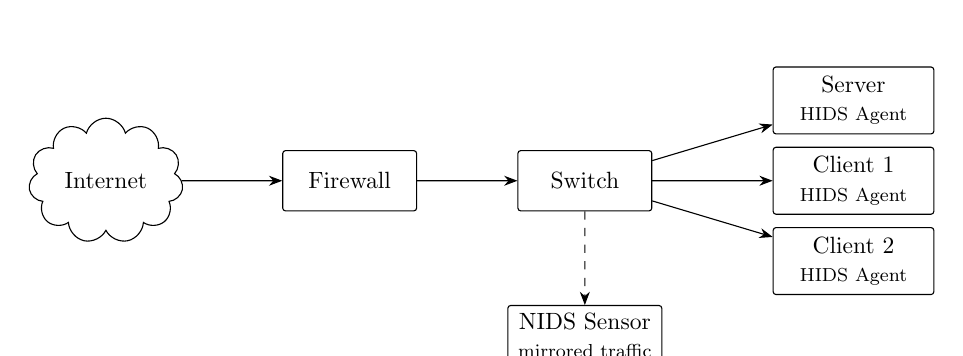
\begin{tikzpicture}[
        scale=0.85, transform shape,
        node distance=1cm and 1.5cm,
        internet/.style={cloud, cloud puffs=11, draw=black, fill=none, aspect=1.4, minimum width=2.1cm, minimum height=1.2cm, align=center},
        device/.style={rectangle, draw=black, fill=none, minimum width=2cm, minimum height=0.9cm, align=center, rounded corners=1pt},
        host/.style={rectangle, draw=black, fill=none, minimum width=2.4cm, minimum height=1cm, align=center, rounded corners=1pt},
        sensor/.style={rectangle, draw=black, fill=none, minimum width=2.3cm, minimum height=0.9cm, align=center, rounded corners=1pt},
        arrow/.style={-Stealth, draw=black},
        mirror/.style={-Stealth, dashed, draw=black}
    ]
        \node[internet] (internet) {Internet};
        \node[device, right=of internet] (fw) {Firewall};
        \node[device, right=of fw] (switch) {Switch};

        \node[host, right=1.8cm of switch, yshift=1.2cm] (server) {Server \\ \footnotesize HIDS Agent};
        \node[host, right=1.8cm of switch] (client1) {Client 1 \\ \footnotesize HIDS Agent};
        \node[host, right=1.8cm of switch, yshift=-1.2cm] (client2) {Client 2 \\ \footnotesize HIDS Agent};
        \node[sensor, below=1.4cm of switch] (nids) {NIDS Sensor \\ \footnotesize mirrored traffic};

        \draw[arrow] (internet) -- (fw);
        \draw[arrow] (fw) -- (switch);
        \draw[arrow] (switch) -- (server);
        \draw[arrow] (switch) -- (client1);
        \draw[arrow] (switch) -- (client2);
        \draw[mirror] (switch) -- (nids);
    \end{tikzpicture}
    \caption{Minh họa vị trí giám sát của NIDS và HIDS}
    \label{fig:nids_hids_position}
\end{figure}

\begin{table}[H]
    \centering
    \renewcommand{\arraystretch}{1.35}
    \begin{tabular}{|>{\raggedright\arraybackslash}p{3cm}|>{\raggedright\arraybackslash}p{5.5cm}|>{\raggedright\arraybackslash}p{6cm}|}
        \hline
        \textbf{Loại hệ thống} & \textbf{Nguồn dữ liệu} & \textbf{Đặc điểm} \\ \hline
        \textbf{NIDS} & Lưu lượng mạng tại switch, gateway hoặc interface giám sát. & Quan sát được nhiều máy trong cùng phân đoạn mạng, phù hợp phát hiện scan, flood và payload độc hại trong lưu lượng không mã hóa. \\ \hline
        \textbf{HIDS} & Log, tiến trình, file và hành vi trên từng máy chủ hoặc endpoint. & Nhìn sâu vào trạng thái máy trạm nhưng cần cài agent trên từng host. \\ \hline
    \end{tabular}
    \caption{Phân loại IDS theo nguồn dữ liệu giám sát}
\end{table}

Hệ thống trong bài tập là một NIDS dạng thụ động: đọc PCAP hoặc sniff interface, phân tích gói tin và ghi cảnh báo ra tệp JSONL.

\section{Phát hiện theo chữ ký và Chỉ số thỏa hiệp IOC}
Phát hiện theo chữ ký là phương pháp đối sánh dữ liệu lưu lượng mạng với một tập hợp các mẫu hoặc luật đã được định nghĩa trước về hành vi độc hại. Các chữ ký này thường được trích xuất từ các Chỉ số thỏa hiệp IOC bao gồm: chuỗi nhị phân đặc trưng của mã độc, địa chỉ IP thuộc mạng botnet, tên miền độc hại của máy chủ điều khiển C2, hoặc các mẫu chuỗi ký tự trong giao thức ứng dụng.

Ưu điểm lớn nhất của phương pháp này là tốc độ xử lý nhanh đối với các cuộc tấn công đã biết, tỷ lệ false positive cực thấp và cung cấp thông tin chi tiết về loại tấn công giúp kiểm chứng dễ dàng. Tuy nhiên, điểm hạn chế chí mạng là hoàn toàn không thể phát hiện các cuộc tấn công Zero-day hoặc các biến thể mã độc đã được thực hiện obfuscation hoặc mã hóa lưu lượng.

Trong dự án này, nhóm đã tự triển khai một công cụ phân tích cú pháp và engine nạp luật tương thích với định dạng luật của Suricata/Snort. Một luật chuẩn bao gồm hai phần:
\begin{itemize}
    \item \textbf{Header:} Khai báo hành động (thường là \texttt{alert}), giao thức mạng (như \texttt{tcp}, \texttt{udp}, \texttt{icmp}, \texttt{dns}, \texttt{http}), dải địa chỉ IP nguồn/đích, cổng dịch vụ nguồn/đích và hướng của luồng dữ liệu (\texttt{->} một chiều, hoặc \texttt{<>} hai chiều).
    \item \textbf{Rule Options:} Được bao quanh bởi dấu ngoặc đơn, chứa các từ khóa điều khiển:
    \begin{itemize}
        \item \texttt{msg}: Chuỗi mô tả thông tin cảnh báo xuất ra log.
        \item \texttt{content}: Chuỗi ký tự nhị phân hoặc văn bản cần tìm kiếm trong gói tin.
        \item \texttt{pcre}: Biểu thức chính quy giúp khớp các mẫu phức tạp hơn.
        \item \texttt{dns.query}: Từ khóa chỉ định vị trí đối sánh thuộc phần truy vấn của giao thức DNS.
        \item \texttt{http.uri}, \texttt{http.method}, \texttt{http.header}: Các sticky buffer chứa dữ liệu HTTP để tăng hiệu năng đối sánh.
        \item \texttt{sid}: Định danh duy nhất cho luật đó.
    \end{itemize}
\end{itemize}

Ví dụ một luật mẫu phát hiện truy vấn tên miền phục vụ kiểm thử độc hại:
\begin{verbatim}
alert dns any any -> any 53 (msg:"Custom DNS Query: example.com";
dns.query; content:"example.com"; nocase; sid:1000101; rev:1;)
\end{verbatim}

\section{Thuật toán so khớp chuỗi trong NIDS}
Trong các hệ thống NIDS dựa trên chữ ký, nhiệm vụ quan trọng nhất và tiêu tốn nhiều tài nguyên CPU nhất là tìm kiếm hàng ngàn chuỗi ký tự độc hại trong phần payload của hàng triệu gói tin đi qua mỗi giây. Để giải quyết bài toán này, các hệ thống IDS/IPS hiện đại như Suricata hay Snort không sử dụng phương pháp duyệt tuần tự thông thường mà áp dụng các thuật toán so khớp chuỗi tối ưu hóa cao:

\subsection{Thuật toán Boyer-Moore}
Thuật toán Boyer-Moore là thuật toán tìm kiếm chuỗi đơn hiệu quả nhất trong thực tế. Khác với thuật toán tìm kiếm thông thường, Boyer-Moore thực hiện so khớp các ký tự từ phải sang trái của mẫu nhưng dịch chuyển mẫu từ trái sang phải trên chuỗi văn bản cần tìm kiếm. 
Thuật toán tận dụng thông tin thu được từ các ký tự không khớp thông qua hai bảng dịch chuyển:
\begin{itemize}
    \item \textbf{Bad Character Rule:} Khi xảy ra lỗi không khớp tại ký tự $T[i] \neq P[j]$, thuật toán sẽ tìm kiếm ký tự $T[i]$ trong mẫu $P$. Nếu có, dịch chuyển mẫu để ký tự $T[i]$ trong mẫu trùng khớp với $T[i]$ trong văn bản. Nếu không có, dịch chuyển toàn bộ mẫu vượt qua vị trí $T[i]$.
    \item \textbf{Good Suffix Rule:} Nếu một phần hậu tố của mẫu khớp với văn bản trước khi xảy ra lỗi không khớp, thuật toán sẽ dịch chuyển mẫu đến vị trí tiếp theo mà hậu tố này xuất hiện lại trong mẫu.
\end{itemize}
Nhờ hai quy tắc này, Boyer-Moore cho phép bỏ qua rất nhiều ký tự trong văn bản mà không cần kiểm tra, đạt độ phức tạp thời gian tốt nhất là $O(n/m)$ với $n$ là độ dài văn bản và $m$ là độ dài mẫu.

\subsection{Thuật toán Aho-Corasick}
Khi số lượng chữ ký tăng lên hàng chục ngàn, việc chạy thuật toán đơn mẫu như Boyer-Moore cho từng chữ ký trên mỗi gói tin sẽ gây ra suy giảm hiệu năng nghiêm trọng. Thuật toán Aho-Corasick giải quyết vấn đề này bằng cách xây dựng một máy trạng thái hữu hạn chứa tất cả các chữ ký cần tìm kiếm.
Máy trạng thái Aho-Corasick hoạt động dựa trên ba hàm cốt lõi:
\begin{itemize}
    \item \textbf{Goto function:} Dẫn dắt quá trình di chuyển từ trạng thái này sang trạng thái khác dựa trên ký tự tiếp theo trong văn bản. Nó tạo ra một cấu trúc cây phân cấp cho tất cả các mẫu.
    \item \textbf{Failure function:} Khi một ký tự không khớp với bất kỳ nhánh con nào tại trạng thái hiện tại, hàm thất bại sẽ chỉ ra trạng thái tiếp theo cần chuyển đến. Hàm này giúp thuật toán không cần phải quay lui trên chuỗi văn bản đầu vào.
    \item \textbf{Output function:} Liên kết các trạng thái với danh sách các mẫu được phát hiện tương ứng khi trạng thái đó được tiếp cận.
\end{itemize}
Nhờ cơ chế này, thuật toán Aho-Corasick có thể tìm kiếm đồng thời tất cả các chữ ký trong văn bản chỉ với một lần duyệt duy nhất. Độ phức tạp thời gian đạt mức tuyến tính $O(n + z)$ trong đó $n$ là độ dài văn bản và $z$ là số lần xuất hiện của các mẫu độc hại, hoàn toàn độc lập với số lượng chữ ký cài đặt. Đây là nền tảng của cơ chế fast\_pattern trong Suricata.

\subsection{Vấn đề quay lui của Biểu thức chính quy và ReDoS}
Mặc dù so khớp chuỗi tĩnh rất nhanh, kẻ tấn công có thể dễ dàng thay đổi một vài ký tự trong payload để né tránh. Do đó, các IDS cần dùng biểu thức chính quy để mô tả các biến thể tấn công linh hoạt hơn. Tuy nhiên, việc sử dụng các công cụ regex truyền thống dựa trên NFA có khả năng gây ra hiện tượng quay lui thảm khốc.
Khi gặp một chuỗi đầu vào không khớp được thiết kế đặc biệt, động cơ regex sẽ thử tất cả các tổ hợp quay lui có thể, dẫn đến độ phức tạp thời gian tăng theo cấp số nhân $O(2^n)$. Kẻ tấn công có thể lợi dụng lỗ hổng này để thực hiện tấn công từ chối dịch vụ vào chính hệ thống IDS. Vì lý do này, các IDS hiện đại thường sử dụng công cụ regex của Google hoạt động dựa trên DFA để đảm bảo thời gian chạy tuyến tính, hoặc hạn chế nghiêm ngặt việc sử dụng các mẫu regex có cấu trúc lặp lồng nhau trong các file luật.

\section{Phát hiện theo hành vi và Cửa sổ trượt}
Khác với phát hiện theo chữ ký tập trung vào một gói tin đơn lẻ, Phát hiện theo hành vi tập trung phân tích xu hướng hoặc mối liên hệ giữa các gói tin theo chuỗi thời gian. Phương pháp này đặc biệt hiệu quả trong việc nhận diện các kiểu tấn công do thám hoặc từ chối dịch vụ vốn không mang nội dung độc hại trong từng gói tin riêng lẻ nhưng lại tạo ra lưu lượng bất thường khi gộp lại.

Để thực hiện điều này một cách tối ưu trong môi trường thời gian thực mà không làm tràn bộ nhớ, kỹ thuật cửa sổ trượt thời gian được áp dụng.
\begin{itemize}
    \item Hệ thống duy trì một hàng đợi hai đầu lưu trữ dấu vết thời gian của các gói tin nhận được từ mỗi địa chỉ IP nguồn trong khoảng thời gian $T$ giây.
    \item Với mỗi gói tin mới đến từ một nguồn, hệ thống tiến hành loại bỏ các bản ghi cũ có $t < t_{\text{current}} - T$ ở đầu hàng đợi.
    \item Sau đó, thêm gói tin hiện tại vào cuối hàng đợi và kiểm tra xem tổng số gói tin hoặc số lượng thuộc tính duy nhất có vượt quá ngưỡng $N$ quy định hay không. Nếu có, phát cảnh báo về hành vi bất thường.
\end{itemize}

Phương pháp này giúp phát hiện được các hành vi nguy hại mà không cần biết trước signature của cuộc tấn công, tuy nhiên thách thức lớn nhất là xác định ngưỡng $N$ và $T$ tối ưu cho từng hạ tầng mạng thực tế. Nếu đặt ngưỡng quá nhạy sẽ dẫn đến báo động giả hàng loạt; ngược lại, nếu đặt ngưỡng quá cao sẽ làm mất tác dụng cảnh báo của hệ thống.

\section{Cơ chế chống lụt cảnh báo bằng thời gian hạ nhiệt}
Trong các đợt tấn công từ chối dịch vụ tốc độ cao hoặc quét cổng quy mô lớn, kẻ tấn công có thể gửi hàng vạn gói tin mỗi giây. Nếu hệ thống NIDS phát sinh cảnh báo cho từng gói tin riêng lẻ, điều này sẽ dẫn đến những hậu quả nghiêm trọng:
\begin{itemize}
    \item \textbf{Tràn ngập cảnh báo:} Hệ thống ghi nhận quá nhiều bản ghi giống nhau trong thời gian ngắn, làm cạn kiệt dung lượng đĩa lưu trữ và gây quá tải hệ thống hiển thị Dashboard.
    \item \textbf{Suy giảm hiệu năng I/O:} Thao tác ghi đĩa liên tục làm chậm toàn bộ tiến trình phân tích gói tin, gây rơi rớt gói tin trên card mạng.
    \item \textbf{Mất tập trung cho quản trị viên:} Quản trị viên an ninh mạng bị quá tải thông tin và khó nhận diện các mối đe dọa khác.
\end{itemize}
Để giải quyết vấn đề này, hệ thống triển khai cơ chế hạ nhiệt cảnh báo thông qua bảng tra cứu thời gian gần nhất của mỗi cặp luật và khóa nguồn. Khi một cảnh báo được kích hoạt, mốc thời gian của nó sẽ được ghi lại. Trong vòng 5 giây tiếp theo, tất cả các cảnh báo trùng lặp từ cùng một nguồn IP cho cùng một luật sẽ bị triệt tiêu hoàn toàn. Cơ chế này giúp gom các sự kiện lặp lại thành một cảnh báo duy nhất mà vẫn đảm bảo tính chính xác về số liệu thống kê gói tin.

\section{Phân tích cấu trúc và tách lọc giao thức HTTP}
Giao thức HTTP là mục tiêu phổ biến của các cuộc tấn công web như SQL Injection hoặc Cross-Site Scripting. Để phân tích hiệu quả lưu lượng HTTP mà không cần tải toàn bộ gói tin thô vào bộ nhớ, hệ thống triển khai bộ phân tích cú pháp HTTP nhỏ gọn hoạt động tại tầng ứng dụng:
\begin{itemize}
    \item Bộ phân tích tiến hành cắt dòng payload thô bằng ký tự xuống dòng CRLF đặc trưng của HTTP.
    \item Dòng đầu tiên được tách để xác định phương thức HTTP và URI yêu cầu.
    \item Các dòng tiếp theo được phân tích theo định dạng khóa-giá trị phân tách bởi dấu hai chấm để trích xuất các trường thông tin quan trọng như Host và User-Agent.
    \item Các trường dữ liệu này sau đó được ánh xạ vào các vùng đệm chuyên biệt trong lớp quản lý bộ đệm sự kiện. Việc tách biệt các vùng đệm này giúp các luật Suricata chỉ thực hiện so khớp trên đúng phân vùng thông tin được yêu cầu, giảm thiểu tối đa các cảnh báo giả do trùng khớp ký tự ngẫu nhiên trong các phần khác của gói tin.
\end{itemize}

\subsection{Cơ chế đối sánh Sticky Buffer và an toàn ứng dụng Web}
Trong NIDS cổ điển, việc đối sánh chữ ký được thực hiện trên toàn bộ payload thô của gói tin. Tuy nhiên, điều này tạo ra một lỗ hổng nghiêm trọng gọi là evasion by misplacement. Kẻ tấn công có thể chèn các chuỗi ký tự độc hại như UNION SELECT vào trong một tiêu đề HTTP không thực thi như Cookie hoặc User-Agent để đánh lừa hệ thống. Máy chủ web khi nhận gói tin sẽ bỏ qua chuỗi này ở tiêu đề và chỉ xử lý URI. Kết quả là NIDS báo động giả hoặc bỏ lọt hành vi tấn công thực sự.

Để khắc phục điều này, NIDS hiện đại thiết lập khái niệm sticky buffer. Khi bộ phân tích cú pháp HTTP hoàn tất việc phân tách gói tin, các dữ liệu được đẩy vào các vùng nhớ đệm riêng biệt gồm:
\begin{itemize}
    \item \texttt{http.method}: Chỉ chứa phương thức yêu cầu như GET, POST, PUT.
    \item \texttt{http.uri}: Chỉ chứa đường dẫn truy cập tài nguyên.
    \item \texttt{http.header}: Chứa toàn bộ phần tiêu đề HTTP.
    \item \texttt{http.user\_agent}: Chứa định danh trình duyệt gửi yêu cầu.
\end{itemize}
Khi một luật Suricata chỉ định từ khóa \texttt{http.uri}, engine đối sánh sẽ chỉ thực hiện tìm kiếm chuỗi trong vùng đệm \texttt{http.uri} chứ không tìm trên toàn bộ gói tin. Cơ chế này loại bỏ hoàn toàn các trường hợp khớp chuỗi nhầm lẫn ở các tiêu đề không liên quan, nâng cao độ chính xác phát hiện lên nhiều lần.

\section{Các kiểu tấn công được mô hình hóa trong bài tập lớn}
Bài tập lớn thực hiện nghiên cứu, mô phỏng và phát hiện 4 dạng tấn công mạng phổ biến dưới góc độ lý thuyết giao thức:

\subsection{Quét cổng}
Quét cổng là giai đoạn do thám đầu tiên trong vòng đời tấn công. Kẻ tấn công gửi các gói tin thăm dò tới một dải cổng dịch vụ của mục tiêu nhằm xác định trạng thái cổng và hệ điều hành của nạn nhân.
Các kỹ thuật quét cổng phổ biến bao gồm:
\begin{itemize}
    \item \textbf{TCP SYN Scan:} Kẻ tấn công gửi gói tin với cờ SYN thiết lập. Nếu nhận được SYN-ACK từ mục tiêu, cổng đó đang mở; kẻ tấn công lập tức gửi gói RST để đóng kết nối thay vì hoàn thành cái bắt tay ba bước. Điều này giúp quét nhanh và tránh bị ghi log bởi các ứng dụng ở tầng trên.
    \item \textbf{TCP FIN Scan:} Gửi gói tin chỉ có cờ FIN. Theo đặc tả giao thức, nếu cổng đóng, hệ điều hành sẽ phản hồi bằng gói RST; nếu cổng mở, hệ điều hành sẽ lờ gói tin đi.
    \item \textbf{TCP NULL Scan và Xmas Scan:} NULL Scan gửi gói tin không bật bất kỳ cờ TCP nào. Xmas Scan bật đồng thời các cờ FIN, PSH, và URG. Cả hai đều lợi dụng phản hồi RST của cổng đóng để xác định trạng thái cổng, vượt qua các bộ lọc tường lửa thô sơ chỉ kiểm tra cờ SYN.
\end{itemize}
Hệ thống phát hiện quét cổng bằng cách theo dõi số lượng cổng đích duy nhất mà một địa chỉ IP nguồn gửi yêu cầu đến trong vòng $T$ giây với các tổ hợp cờ TCP tương ứng.

\subsection{Tấn công từ chối dịch vụ ICMP Flood}
ICMP Flood là hình thức tấn công từ chối dịch vụ cổ điển. Kẻ tấn công gửi liên tục các gói tin truy vấn ICMP Echo Request tới địa chỉ IP của nạn nhân với tốc độ cực cao nhằm làm nghẽn băng thông đường truyền hoặc khiến CPU của thiết bị mạng bị quá tải do phải xử lý và phản hồi liên tục bằng gói tin ICMP Echo Reply.
Hệ thống phát hiện bằng cách đếm số lượng gói tin ICMP truy vấn từ một địa chỉ nguồn trong cửa sổ trượt. Việc loại trừ các gói tin ICMP Reply ra khỏi bộ đếm là cực kỳ quan trọng để tránh tình trạng báo động giả lên chính nạn nhân khi họ đang gửi phản hồi lại kẻ tấn công.

\subsection{Tấn công từ chối dịch vụ TCP SYN Flood}
TCP SYN Flood lợi dụng cơ chế hàng đợi kết nối nửa mở backlog queue trong quá trình bắt tay ba bước của giao thức TCP.
Mô hình lý thuyết của cuộc tấn công diễn ra qua bốn bước sau:
\begin{enumerate}
    \item Kẻ tấn công gửi liên tục các gói tin SYN yêu cầu kết nối với địa chỉ IP nguồn giả mạo hoặc không tồn tại.
    \item Máy chủ nạn nhân tiếp nhận, đưa kết nối vào hàng đợi kết nối nửa mở backlog queue, chuyển trạng thái kết nối sang SYN-RECEIVED và phản hồi bằng gói SYN-ACK tới địa chỉ IP nguồn giả mạo đó.
    \item Do địa chỉ IP nguồn là giả mạo, máy chủ sẽ không bao giờ nhận được gói tin phản hồi ACK cuối cùng từ kẻ tấn công để hoàn tất kết nối. Kết nối nửa mở này sẽ được lưu giữ trong hàng đợi cho đến khi hết thời gian chờ timeout.
    \item Khi kẻ tấn công gửi hàng vạn gói tin SYN liên tục, hàng đợi kết nối nửa mở của máy chủ sẽ nhanh chóng bị lấp đầy, khiến máy chủ từ chối mọi yêu cầu kết nối TCP hợp lệ khác từ người dùng thông thường.
\end{enumerate}
NIDS phát hiện cuộc tấn công này bằng cách theo dõi tần suất các gói tin chỉ bật cờ SYN mà không bật cờ ACK nhắm tới một dịch vụ cụ thể trên máy chủ mục tiêu.

\subsection{Kênh truyền độc hại qua DNS}
DNS Tunneling là kỹ thuật đóng gói lưu lượng của giao thức khác vào trong các gói tin DNS hợp lệ nhằm vượt qua các thiết bị kiểm soát biên. Vì DNS là dịch vụ cốt lõi bắt buộc phải mở trên tường lửa để phân giải tên miền, kẻ tấn công có thể lợi dụng điều này để rò rỉ dữ liệu hoặc duy trì kênh kết nối ẩn.
Cơ chế hoạt động dựa trên cấu trúc phân cấp DNS: kẻ tấn công đăng ký một tên miền và trỏ bản ghi Name Server về một máy chủ điều khiển do chúng kiểm soát. Khi mã độc gửi truy vấn phân giải tên miền phụ chứa dữ liệu mã hóa, truy vấn này sẽ được chuyển tiếp qua các DNS Resolver hợp lệ trên Internet và cuối cùng gửi tới máy chủ điều khiển của kẻ tấn công. Máy chủ điều khiển sẽ trích xuất phần tên miền phụ để đọc dữ liệu và phản hồi lại mã độc dưới dạng các bản ghi DNS TXT, CNAME, hoặc A chứa lệnh điều khiển mới.

Hệ thống phát hiện DNS Tunneling thông qua các dấu hiệu bất thường của chuỗi truy vấn DNS:
\begin{itemize}
    \item \textbf{Độ dài truy vấn query\_length:} Tên miền phụ chứa dữ liệu đóng gói thường có độ dài rất lớn. Giao thức DNS giới hạn tổng độ dài truy vấn tối đa là 253 ký tự.
    \item \textbf{Độ dài nhãn lớn nhất max\_label\_length:} Mỗi nhãn phân tách bởi dấu chấm có độ dài lớn, giới hạn tối đa là 63 ký tự cho mỗi nhãn theo đặc tả RFC.
    \item \textbf{Độ hỗn loạn thông tin Shannon Entropy:} Các tên miền thông thường được đặt theo ngôn ngữ tự nhiên nên có tính lặp lại cao và độ hỗn loạn thấp. Ngược lại, dữ liệu mã hóa độc hại như Base32 hay Base64 có tính ngẫu nhiên rất lớn. Công thức toán học tính Entropy Shannon của một chuỗi ký tự $S$ là:
    $$H(S) = - \sum_{i=1}^{n} P(x_i) \log_2 P(x_i)$$
    Trong đó $P(x_i)$ là tần suất xuất hiện của ký tự thứ $x_i$ trong chuỗi $S$. Một tên miền phụ có độ dài nhãn lớn và entropy vượt quá ngưỡng $3.8$ liên tục sẽ bị hệ thống đưa vào diện nghi vấn DNS Tunneling.
\end{itemize}

\section{Giới hạn lý thuyết của việc triển khai NIDS}
Mặc dù NIDS là công cụ quan trọng, trên khía cạnh lý thuyết và thực tiễn triển khai vẫn tồn tại các giới hạn sau:
\begin{itemize}
    \item \textbf{Mã hóa lưu lượng:} Khi các giao thức chuyển dịch sang HTTPS, DoT, DoH, NIDS hoàn toàn không thể đọc được nội dung của gói tin để thực hiện đối sánh chữ ký nếu không có giải pháp giải mã trung gian.
    \item \textbf{Thiếu khả năng lắp ráp luồng dữ liệu:} Các cuộc tấn công ứng dụng có thể được kẻ tấn công chia nhỏ payload qua nhiều phân đoạn TCP. Nếu NIDS phân tích từng gói tin độc lập mà không tái cấu trúc lại luồng dữ liệu TCP, hệ thống sẽ không phát hiện ra mã độc.
    \item \textbf{Kỹ thuật né tránh:} Kẻ tấn công có thể gửi các gói tin có thời gian sống khác nhau hoặc chồng chéo dữ liệu khiến NIDS nhận dạng một đằng nhưng hệ điều hành của nạn nhân lại xử lý một nẻo, dẫn đến việc bỏ lọt tấn công.
    \item \textbf{Hiệu năng phần cứng và ngôn ngữ:} Việc sử dụng các ngôn ngữ bậc cao như Python kết hợp thư viện Scapy rất tốt cho việc nghiên cứu thử nghiệm học thuật, tuy nhiên trong môi trường mạng doanh nghiệp thực tế với băng thông lớn, hệ thống sẽ gặp hiện tượng nghẽn cổ chai CPU và rơi gói tin hàng loạt. Các hệ thống thực tế phải sử dụng C/C++/Rust kết hợp các cơ chế bắt gói tin hiệu năng cao.
\end{itemize}

\chapter{Kiến trúc và Triển khai Hệ thống NIDS}

\section{Tổng quan kiến trúc}
Hệ thống NIDS được xây dựng bằng Python 3 và tổ chức theo mô hình pipeline. Mỗi gói tin sau khi được đọc từ PCAP hoặc interface mạng sẽ đi qua các bước: thu thập, chuẩn hóa, phát hiện, lưu trữ và hiển thị.

\begin{enumerate}
    \item \textbf{Capture:} đọc gói tin bằng Scapy từ tệp PCAP hoặc giao diện mạng.
    \item \textbf{Parser:} chuyển gói tin Scapy thành đối tượng \texttt{PacketEvent}.
    \item \textbf{Detection Engine:} chạy luật hành vi/anomaly và luật chữ ký.
    \item \textbf{Storage:} ghi cảnh báo ra tệp JSONL.
    \item \textbf{Dashboard:} đọc dữ liệu cảnh báo và hiển thị thống kê bằng Flask.
\end{enumerate}

\begin{figure}[h!]
    \centering
    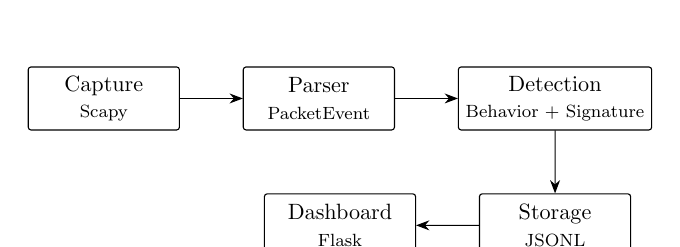
\begin{tikzpicture}[
        scale=0.8, transform shape,
        node distance=1cm and 1cm,
        box/.style={rectangle, draw=black, fill=none, minimum width=2.4cm, minimum height=1cm, align=center, rounded corners=1pt},
        arrow/.style={-Stealth, draw=black}
    ]
        \node[box] (capture) {Capture \\ \footnotesize Scapy};
        \node[box, right=of capture] (parser) {Parser \\ \footnotesize PacketEvent};
        \node[box, right=of parser] (engine) {Detection \\ \footnotesize Behavior + Signature};
        \node[box, below=of engine] (storage) {Storage \\ \footnotesize JSONL};
        \node[box, left=of storage] (dashboard) {Dashboard \\ \footnotesize Flask};

        \draw[arrow] (capture) -- (parser);
        \draw[arrow] (parser) -- (engine);
        \draw[arrow] (engine) -- (storage);
        \draw[arrow] (storage) -- (dashboard);
    \end{tikzpicture}
    \caption{Luồng dữ liệu của hệ thống NIDS}
    \label{fig:nids_architecture}
\end{figure}

\section{Thu thập và chuẩn hóa gói tin}
\subsection{Capture}
Module \texttt{nids/capture.py} cung cấp hai cách lấy dữ liệu: đọc từ tệp PCAP và sniff trực tiếp trên interface. Với live capture, Scapy gọi callback cho từng gói tin; nếu parser chuyển đổi thành công thì sự kiện sẽ được đưa vào detection engine.

\begin{lstlisting}[language=Python, caption={Live capture bằng Scapy}]
def sniff_live(interface: str, callback: PacketCallback, limit: int = 0) -> None:
    from scapy.all import sniff

    def handle_packet(packet: object) -> None:
        event = packet_to_event(packet)
        if event is not None:
            callback(event)

    sniff(iface=interface, prn=handle_packet, store=False, count=limit)
\end{lstlisting}

\subsection{PacketEvent}
Raw packet chứa nhiều trường phụ thuộc giao thức nên khó xử lý trực tiếp trong rule engine. Vì vậy, module \texttt{nids/parser.py} chuẩn hóa các trường cần thiết thành \texttt{PacketEvent}: thời gian, IP nguồn/đích, cổng nguồn/đích, giao thức, TCP flags, ICMP type, DNS query, payload text và các trường HTTP phổ biến.

\begin{lstlisting}[language=Python, caption={Cấu trúc PacketEvent}]
@dataclass(frozen=True)
class PacketEvent:
    timestamp: float
    src_ip: str | None
    dst_ip: str | None
    src_port: int | None
    dst_port: int | None
    protocol: str
    length: int
    tcp_flags: str | None = None
    icmp_type: int | None = None
    dns_query: str | None = None
    payload_text: str | None = None
    http_method: str | None = None
    http_uri: str | None = None
    http_host: str | None = None
    http_user_agent: str | None = None
\end{lstlisting}

Payload được giới hạn kích thước khi chuyển thành chuỗi để tránh tốn bộ nhớ và giảm chi phí so khớp. Đây là lựa chọn phù hợp cho demo, nhưng cũng là một giới hạn khi phân tích payload lớn hoặc payload bị chia nhỏ.

\section{Detection Engine}
Module \texttt{nids/engine.py} đóng vai trò điều phối. Mỗi \texttt{PacketEvent} được đếm vào thống kê giao thức, sau đó gửi đến \texttt{SlidingWindowRules}. Các cảnh báo sinh ra được ghi xuống \texttt{AlertStore}.

\begin{lstlisting}[language=Python, caption={Luồng xử lý một sự kiện}]
def process_event(self, event: PacketEvent) -> list[Alert]:
    self.packet_count += 1
    self.protocol_counts[event.protocol] += 1

    alerts = self.rules.evaluate(event)
    self.store.append_many(alerts)
    self.alert_count += len(alerts)
    return alerts
\end{lstlisting}


\section{Luật phát hiện tích hợp}
Các luật hành vi và anomaly được triển khai bằng cửa sổ trượt theo thời gian. Hệ thống lưu các sự kiện gần nhất theo IP nguồn và loại bỏ dữ liệu đã nằm ngoài khung thời gian cấu hình. Các ngưỡng trong bảng là giá trị lab/demo, chưa phải khuyến nghị production.

Để lưu giữ vết thời gian (timestamps) của các gói tin trong cửa sổ trượt thời gian một cách tối ưu, hệ thống sử dụng hàng đợi hai đầu (\texttt{collections.deque}) thay vì danh sách thông thường (\texttt{list}).
\begin{itemize}
    \item \textbf{Hiệu năng chèn và xóa:} Việc loại bỏ các gói tin cũ ở đầu hàng đợi đòi hỏi thao tác xóa ở đầu. Đối với Python \texttt{list}, thao tác \texttt{pop(0)} có độ phức tạp thời gian là $O(N)$ do phải dịch chuyển toàn bộ phần tử còn lại trong bộ nhớ. Đối với \texttt{deque}, thao tác \texttt{popleft()} chỉ mất thời gian $O(1)$, giúp hệ thống duy trì hiệu suất xử lý gói tin cực cao ở thời gian thực.
    \item \textbf{Thuật toán loại bỏ phần tử hết hạn:}
\end{itemize}

\begin{lstlisting}[language=Python, caption={Loại bỏ sự kiện cũ trong cửa sổ thời gian}]
@staticmethod
def _drop_old_times(window: deque[float], now: float, seconds: int) -> None:
    while window and now - window[0] > seconds:
        window.popleft()
\end{lstlisting}

\subsection{Cơ chế chống tấn công cạn kiệt bộ nhớ (State Exhaustion DoS)}
Một trong những điểm yếu lớn nhất của các hệ thống IDS/IPS lưu vết trạng thái (stateful) là nguy cơ bị tấn công **Cạn kiệt trạng thái (State Exhaustion)**. Kẻ tấn công có thể giả mạo hàng triệu địa chỉ IP nguồn ngẫu nhiên để gửi gói tin qua NIDS. Nếu hệ thống tự động khởi tạo hàng đợi mới cho mỗi IP nguồn mà không có cơ chế dọn dẹp, bộ nhớ RAM của hệ thống sẽ nhanh chóng bị lấp đầy và dẫn đến sập toàn bộ NIDS (Denial of Service).

Để giải quyết vấn đề bảo mật này, hệ thống triển khai một thuật toán dọn dẹp theo phong cách LRU (Least Recently Used) định kỳ sau mỗi 1000 gói tin được xử lý:
\begin{itemize}
    \item Hệ thống đặt giới hạn số lượng nguồn theo dõi tối đa là $10.000$ địa chỉ nguồn thông qua biến \texttt{\_max\_tracked\_sources}.
    \item Khi số lượng nguồn theo dõi vượt quá giới hạn này, hàm \texttt{\_cleanup\_tracked\_sources} sẽ tiến hành sắp xếp các địa chỉ IP theo mốc thời gian hoạt động gần nhất của chúng.
    \item Hệ thống sau đó tự động giải phóng (xóa bỏ) một nửa số lượng địa chỉ nguồn ít hoạt động nhất (được ghi nhận mốc thời gian cũ nhất) để nhường chỗ cho các nguồn mới, đảm bảo dung lượng bộ nhớ RAM luôn nằm trong tầm kiểm soát an toàn.
\end{itemize}

Các luật tích hợp gồm:

\begin{table}[H]
    \centering
    \scriptsize
    \renewcommand{\arraystretch}{1.3}
    \begin{tabular}{|>{\raggedright\arraybackslash}p{1.5cm}|>{\raggedright\arraybackslash}p{2.5cm}|>{\raggedright\arraybackslash}p{2.5cm}|>{\raggedright\arraybackslash}p{4.9cm}|>{\raggedright\arraybackslash}p{1.3cm}|}
        \hline
        \textbf{Rule ID} & \textbf{Attack} & \textbf{Nhóm phát hiện} & \textbf{Điều kiện mặc định} & \textbf{Severity} \\ \hline
        RULE-001 & Port Scan & Behavior-based & $\geq$ 20 TCP destination ports từ một source trong 10 giây. & Medium \\ \hline
        RULE-002 & ICMP Ping Flood & Behavior-based & $\geq$ 100 ICMP request packets trong 10 giây. & High \\ \hline
        RULE-003 & TCP SYN Flood & Behavior-based & $\geq$ 100 TCP SYN packets without ACK trong 10 giây. & High \\ \hline
        RULE-004 & DNS Tunneling & \makecell[l]{Behavior/\\anomaly-based} & $\geq$ 5 DNS query đáng ngờ từ cùng source trong 30 giây. & Medium \\ \hline
    \end{tabular}
    \caption{Các detection rules tích hợp trong prototype}
\end{table}

Với port scan, prototype chỉ đếm các probe flags như SYN, FIN, NULL và Xmas. Xmas scan tương ứng FIN + PSH + URG. ACK scan có thể tạo false positive nếu không có state tracking đầy đủ, vì vậy phần phát hiện ACK scan chỉ nên xem là minh họa trong prototype.

\section{Luật chữ ký dạng Suricata-style subset}
Ngoài luật hành vi, hệ thống hỗ trợ một tập con cú pháp kiểu Suricata/Snort. Người dùng có thể truyền tệp luật qua tham số \texttt{--rules}. Trong lần thử nghiệm được lưu ở \texttt{data/alerts.jsonl}, luật chữ ký được kích hoạt là luật DNS kiểm tra truy vấn chứa \texttt{example.com}:

\begin{lstlisting}[language=bash, breaklines=true, caption={Luật chữ ký dùng trong demo}]
alert dns any any -> any 53 (msg:"Custom DNS Query: example.com"; dns.query; content:"example.com"; nocase; classtype:policy-violation; priority:3; sid:1000101; rev:1;)
\end{lstlisting}

Mục tiêu của phần này là minh họa cách một signature engine hoạt động: phân tích header luật, chọn buffer cần kiểm tra, sau đó so khớp nội dung hoặc biểu thức chính quy. Đây là \textit{Suricata-style subset}, không phải engine tương thích đầy đủ với Suricata/Snort.

Subset prototype hỗ trợ các thành phần cơ bản như header luật, \texttt{content}, \texttt{pcre}, \texttt{nocase}, một số sticky buffer DNS/payload và threshold đơn giản. Các tính năng chưa hỗ trợ đầy đủ gồm \texttt{depth/offset}, \texttt{distance/within}, \texttt{byte\_test}, \texttt{flowbits}, TCP stream inspection, \texttt{file\_data} và tối ưu \texttt{fast\_pattern}. Tùy chọn \texttt{flow} hiện chỉ được kiểm tra ở mức hướng cơ bản, chưa phải stateful TCP flow tracking như IDS production.


\section{Lưu trữ và Dashboard hiển thị}
\subsection{Lưu trữ cảnh báo dạng Append-Only JSON Lines (JSONL)}
Hệ thống sử dụng định dạng tệp JSON Lines (JSONL) thông qua lớp \texttt{AlertStore} để lưu trữ nhật ký cảnh báo. Mỗi cảnh báo mới xuất hiện sẽ được mã hóa thành một chuỗi JSON độc lập và kết thúc bằng ký tự xuống dòng (\texttt{\textbackslash n}).
Quyết định thiết kế này dựa trên các đặc tính kỹ thuật quan trọng liên quan đến hiệu năng hệ thống:
\begin{itemize}
    \item \textbf{Độ phức tạp ghi tối ưu $O(1)$:} Đối với định dạng JSON chuẩn (trong đó toàn bộ file là một mảng lớn \texttt{[]}), mỗi khi có cảnh báo mới, hệ thống bắt buộc phải đọc toàn bộ nội dung file cũ vào bộ nhớ RAM, phân tích cú pháp sang kiểu dữ liệu danh sách của Python, thêm phần tử mới, chuyển đổi lại thành chuỗi JSON và ghi đè toàn bộ tệp tin lên đĩa cứng. Thao tác này có độ phức tạp thời gian tăng dần theo độ lớn của lịch sử cảnh báo $O(M)$. Ngược lại, đối với JSONL, hệ thống chỉ cần mở tệp ở chế độ ghi tiếp (append mode - \texttt{"a"}) và ghi trực tiếp dòng mới vào cuối tệp tin mà không cần quan tâm đến kích thước hiện tại của tệp. Thao tác này luôn đạt độ phức tạp $O(1)$.
    \item \textbf{Độ tin cậy và Khôi phục:} Trong trường hợp hệ thống NIDS bị sập đột ngột (ví dụ mất điện, lỗi crash), các dòng cảnh báo đã ghi trước đó vẫn hoàn toàn nguyên vẹn và không bị lỗi cấu trúc tệp tin (corrupted file) như khi ghi tệp tin JSON thông thường (vốn dễ bị thiếu dấu ngoặc đóng cuối tệp).
    \item \textbf{Tương thích hệ thống lớn:} Định dạng JSONL là định dạng chuẩn được hỗ trợ mặc định bởi các tác nhân thu thập log nổi tiếng như Filebeat, Fluentd hoặc Logstash để đẩy dữ liệu về hệ thống SIEM tập trung.
\end{itemize}

\subsection{Cơ chế hiển thị trên Dashboard Flask}
Dashboard được xây dựng dựa trên framework Flask (\texttt{dashboard/app.py}). Để đảm bảo Dashboard luôn hiển thị thông tin trực quan mà không tạo ra gánh nặng I/O đọc tệp tin liên tục cho ổ cứng máy chủ, hệ thống áp dụng cơ chế tối ưu hóa sau:
\begin{itemize}
    \item \textbf{Cache theo mốc thời gian sửa đổi (File stat):} Trước khi thực hiện đọc và phân tích tệp tin \texttt{alerts.jsonl}, ứng dụng web kiểm tra thuộc tính mốc thời gian sửa đổi cuối cùng của tệp tin (\texttt{os.path.getmtime}). Nếu tệp tin không có thay đổi so với lần đọc trước, Dashboard sẽ trả về ngay kết quả đã được cache sẵn trong bộ nhớ RAM mà không cần thực hiện thao tác I/O đọc ổ cứng.
    \item \textbf{Phân tích thống kê thời gian thực:} Khi phát hiện tệp tin cảnh báo có sự thay đổi, Dashboard thực hiện đọc tệp, trích xuất dữ liệu để tính toán nhanh:
    \begin{itemize}
        \item Tổng số lượng cảnh báo đã kích hoạt.
        \item Biểu đồ thống kê số lượng cảnh báo phân nhóm theo mức độ nghiêm trọng (\texttt{severity}: High, Medium, Low).
        \item Phân tích danh sách các địa chỉ IP nguồn xuất hiện nhiều nhất (\texttt{Top Attacker IPs}) hỗ trợ khoanh vùng mối đe dọa.
        \item Danh sách hiển thị chi tiết mười cảnh báo gần nhất bao gồm đầy đủ bằng chứng (\texttt{evidence}) thu thập được từ gói tin.
    \end{itemize}
\end{itemize}
Dashboard phục vụ quan sát và trình diễn kết quả; phần phản ứng tự động như chặn IP hoặc cập nhật tường lửa chưa nằm trong phạm vi bài tập.

\chapter{Kịch bản Thử nghiệm và Đánh giá}

\section{Môi trường thử nghiệm}
Việc kiểm thử được thực hiện trong môi trường lab ảo hóa để tránh ảnh hưởng đến mạng thật. Mô hình gồm ba thành phần:

\begin{itemize}
    \item \textbf{Host Machine:} chạy NIDS engine và Flask dashboard.
    \item \textbf{Kali Linux VM:} đóng vai trò máy tạo lưu lượng kiểm thử bằng \texttt{nmap}, \texttt{hping3}, \texttt{dig} và \texttt{curl}.
    \item \textbf{Target VM:} nhận lưu lượng scan, flood, DNS và HTTP. Target cần có dịch vụ HTTP ở cổng 80 để kiểm thử luật chữ ký web.
\end{itemize}

\begin{figure}[h!]
    \centering
    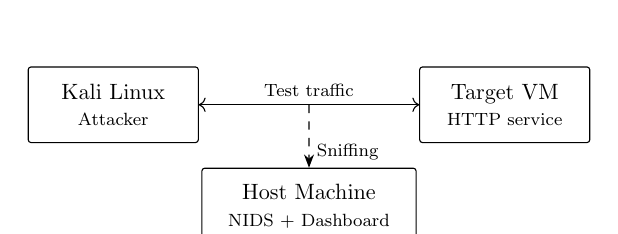
\begin{tikzpicture}[
        scale=0.8, transform shape,
        node distance=1.5cm and 3.5cm,
        machine/.style={rectangle, draw=black, fill=none, minimum width=2.7cm, minimum height=1.2cm, align=center, rounded corners=1pt},
        nids/.style={rectangle, draw=black, fill=none, minimum width=3.4cm, minimum height=1.2cm, align=center, rounded corners=1pt},
        arrow/.style={-Stealth, dashed, draw=black}
    ]
        \node[machine] (kali) {Kali Linux \\ \footnotesize Attacker};
        \node[machine, right=of kali] (target) {Target VM \\ \footnotesize HTTP service};
        \node[nids, below=1cm of $(kali)!0.5!(target)$] (host) {Host Machine \\ \footnotesize NIDS + Dashboard};

        \draw[<->, draw=black] (kali) -- node[above, font=\footnotesize] {Test traffic} (target);
        \draw[arrow] ($(kali)!0.5!(target)$) -- node[right, near end, font=\footnotesize] {Sniffing} (host);
    \end{tikzpicture}
    \caption{Mô hình lab kiểm thử}
    \label{fig:test_environment}
\end{figure}

\section{Khởi động hệ thống}
Trên host, dashboard được chạy ở một terminal:

\begin{lstlisting}[language=bash, caption={Khởi động dashboard}]
python3 dashboard/app.py
\end{lstlisting}

NIDS engine được chạy ở terminal khác. Interface cần thay bằng interface thực tế kết nối các máy ảo:

\begin{lstlisting}[language=bash, caption={Khởi động NIDS engine}]
sudo .venv/bin/python main.py --iface <YOUR_INTERFACE> --rules custom.rules --limit 0
\end{lstlisting}

Khi dùng PCAP thay cho live capture, có thể chạy:

\begin{lstlisting}[language=bash, caption={Phân tích PCAP}]
python3 main.py --pcap sample.pcap --rules custom.rules
\end{lstlisting}

\section{Các kịch bản kiểm thử}
\subsection{Quét cổng bằng nmap}
Kịch bản sử dụng \texttt{nmap} để gửi SYN tới nhiều cổng đích trong thời gian ngắn:

\begin{lstlisting}[language=bash]
nmap -sS -p 21,22,23,25,53,80,110,135,139,143,443,445,\
993,995,1433,1723,3306,3389,5900,8080,8443,8888,9090,\
9200,9300 --min-rate 300 -T4 -n --open <TARGET_IP>
\end{lstlisting}

Kết quả mong đợi là cảnh báo \textbf{RULE-001 Port Scan}, vì cùng một IP nguồn truy cập nhiều cổng TCP đích trong cửa sổ 10 giây.

\subsection{ICMP Ping Flood}
Kịch bản gửi nhiều gói ICMP Echo Request:

\begin{lstlisting}[language=bash]
hping3 --icmp -c 120 -i u5000 <TARGET_IP>
\end{lstlisting}

Kết quả mong đợi là cảnh báo \textbf{RULE-002 ICMP Ping Flood} khi bộ đếm ICMP từ cùng nguồn vượt ngưỡng.

\subsection{TCP SYN Flood}
Kịch bản gửi nhiều gói SYN tới cổng 80:

\begin{lstlisting}[language=bash]
hping3 -S -p 80 -c 120 -i u5000 <TARGET_IP>
\end{lstlisting}

Kết quả mong đợi là cảnh báo \textbf{RULE-003 TCP SYN Flood}. Trong phạm vi đồ án, hệ thống chỉ cảnh báo dựa trên số lượng gói SYN, chưa kiểm tra trạng thái hoàn tất kết nối ở mức TCP stream đầy đủ.

\subsection{DNS đáng ngờ và DNS tunneling}
Kịch bản DNS gồm hai nhóm: truy vấn tên miền nằm trong danh sách đáng ngờ và truy vấn có nhãn dài/entropy cao.

\begin{lstlisting}[language=bash]
dig malware.test
dig aGVsbG93b3JsZGhlbGxvd2...tunnel.example.com
\end{lstlisting}

Kết quả mong đợi là \textbf{RULE-004 Suspicious DNS Query} với tên miền đáng ngờ và \textbf{RULE-005 DNS Tunneling Suspicion} khi có đủ số truy vấn bất thường trong cửa sổ thời gian.

\subsection{HTTP signature rules}
Các request HTTP được dùng để kiểm tra luật chữ ký:

\begin{lstlisting}[language=bash]
curl -s "http://<TARGET_IP>/index.php?id=%27%20OR%20%271%27%3D%271"
curl -A "sqlmap/1.7.8#stable" "http://<TARGET_IP>/"
curl -s -X POST "http://<TARGET_IP>/login" \
  --data "username=admin&password=%27+OR+%271%27%3D%271"
\end{lstlisting}

Kết quả mong đợi là các cảnh báo từ luật \texttt{custom.rules}: SQL Injection trong URI, User-Agent chứa \texttt{sqlmap}, và SQL Injection trong body POST.

\section{Đánh giá kết quả}
Trong môi trường lab, các kịch bản trên kiểm tra được cả hai lớp phát hiện:

\begin{itemize}
    \item Luật hành vi phát hiện các mẫu dựa trên tần suất và số lượng sự kiện trong thời gian ngắn.
    \item Luật chữ ký phát hiện các chuỗi đặc trưng trong HTTP và payload thô.
    \item Dashboard hiển thị được số lượng cảnh báo, mức độ nghiêm trọng, IP nguồn và danh sách cảnh báo gần nhất.
\end{itemize}

Kết quả này xác nhận hệ thống đáp ứng mục tiêu học tập và trình diễn. Tuy nhiên, đánh giá này chỉ có giá trị trong phạm vi lab có kiểm soát. Để kết luận về độ chính xác trong mạng thực tế cần có bộ dữ liệu lớn hơn, lưu lượng nền đa dạng hơn, kiểm thử false positive/false negative và đo hiệu năng xử lý gói tin.

\chapter{Kết luận và Hướng phát triển}

\section{Kết quả đạt được}
Đồ án đã xây dựng được một hệ thống NIDS nhỏ gọn phục vụ học tập và trình diễn. Hệ thống hoàn chỉnh các thành phần chính của một pipeline phát hiện xâm nhập mạng:

\begin{itemize}
    \item Đọc lưu lượng từ PCAP hoặc live interface bằng Scapy.
    \item Chuẩn hóa packet thành cấu trúc \texttt{PacketEvent}.
    \item Phát hiện hành vi bằng cửa sổ trượt thời gian.
    \item Phân tích một tập con luật Suricata để phát hiện chữ ký trong HTTP, DNS và payload.
    \item Ghi cảnh báo ra JSON Lines và hiển thị qua dashboard Flask.
    \item Có kịch bản demo để kiểm tra các rule chính trong môi trường lab.
\end{itemize}

Kết quả quan trọng nhất của đồ án là làm rõ cách các thành phần IDS phối hợp với nhau: capture cung cấp dữ liệu, parser chuẩn hóa dữ liệu, rule engine tạo cảnh báo, storage lưu lại kết quả và dashboard hỗ trợ quan sát.

\section{Hạn chế}
Hệ thống hiện tại vẫn có một số hạn chế kỹ thuật:

\begin{itemize}
    \item \textbf{Chỉ phát hiện, chưa ngăn chặn:} hệ thống không chặn gói tin, không reset kết nối và không tự động cập nhật tường lửa.
    \item \textbf{Chưa xử lý lưu lượng mã hóa:} nội dung HTTPS/TLS không thể được kiểm tra bằng chữ ký nếu không có cơ chế giải mã hợp lệ.
    \item \textbf{Chưa tái tạo TCP stream đầy đủ:} payload bị chia nhỏ qua nhiều gói tin có thể làm giảm hiệu quả của signature matching.
    \item \textbf{Hiệu năng còn giới hạn:} Python và Scapy phù hợp cho demo, nhưng chưa phù hợp với môi trường có lưu lượng lớn nếu không tối ưu thêm.
    \item \textbf{Phụ thuộc vào ngưỡng và luật:} chất lượng cảnh báo phụ thuộc vào cấu hình threshold và độ đầy đủ của tập luật chữ ký.
\end{itemize}

\section{Hướng phát triển}
Các hướng cải tiến phù hợp với kiến trúc hiện tại gồm:

\begin{itemize}
    \item Bổ sung TCP stream reassembly để kiểm tra payload ở mức phiên thay vì từng gói riêng lẻ.
    \item Mở rộng parser HTTP/DNS và tăng mức tương thích với cú pháp Suricata.
    \item Thêm cơ chế cấu hình rule và threshold qua tệp YAML hoặc giao diện dashboard.
    \item Đo hiệu năng trên PCAP lớn và tối ưu luồng xử lý để giảm packet drop.
    \item Tích hợp phản ứng bán tự động như xuất IOC, webhook hoặc cập nhật danh sách chặn cho firewall trong môi trường lab.
    \item Xây dựng bộ kiểm thử với cả traffic bình thường và traffic tấn công để đánh giá false positive/false negative rõ ràng hơn.
\end{itemize}

\section{Kết luận}
Hệ thống đã đáp ứng mục tiêu chính của đồ án: minh họa được một NIDS hoạt động từ khâu thu thập gói tin đến sinh cảnh báo và trực quan hóa kết quả. Dù chưa phải hệ thống production, đồ án cung cấp nền tảng thực hành tốt để hiểu các kỹ thuật phát hiện xâm nhập mạng và các giới hạn khi triển khai IDS trong thực tế.

% \clearpage
\chapter*{Phụ lục}
\addcontentsline{toc}{chapter}{Phụ lục}

\section*{Phụ lục A: Hướng dẫn cài đặt và cấu hình hệ thống}
Để triển khai và chạy thử nghiệm hệ thống NIDS trong môi trường thực tế hoặc phòng thí nghiệm, người sử dụng cần thực hiện các bước cấu hình hệ điều hành và cài đặt môi trường như sau:

\subsection*{1. Cài đặt các thư viện phụ thuộc của hệ thống}
Hệ thống yêu cầu cài đặt phiên bản Python 3.8 trở lên. Các thư viện phụ thuộc được quản lý thông qua tệp tin \texttt{requirements.txt} và có thể cài đặt bằng trình quản lý gói pip:
\begin{lstlisting}[language=bash]
# Tao moi moi truong ao python
python3 -m venv .venv

# Kich hoat moi truong ao tren Linux/macOS
source .venv/bin/activate

# Kich hoat moi truong ao tren Windows
.venv\Scripts\activate

# Cap nhat pip va cai dat cac thu vien phu thuoc
pip install --upgrade pip
pip install -r requirements.txt
\end{lstlisting}

\subsection*{2. Cấu hình quyền bắt gói tin trực tiếp trên Linux}
Giao thức bắt gói tin trực tiếp trên card mạng yêu cầu tiến trình chạy dưới quyền quản trị tối cao root. Nếu chạy bằng tài khoản thông thường, thư viện Scapy sẽ báo lỗi không thể truy cập socket thô của hệ thống.
\begin{lstlisting}[language=bash]
# Chay engine NIDS voi quyen sudo tren Linux
sudo .venv/bin/python main.py --iface eth0 --rules custom.rules
\end{lstlisting}

Để bắt gói tin ở chế độ promiscuous mode nhằm giám sát toàn bộ lưu lượng trong phân đoạn mạng chứ không chỉ các gói tin gửi trực tiếp đến máy chủ, ta cần kích hoạt tính năng này trên card mạng đích:
\begin{lstlisting}[language=bash]
# Kich hoat promiscuous mode cho card mang eth0
sudo ip link set eth0 promisc on
\end{lstlisting}

\subsection*{3. Cấu hình hỗ trợ trên Windows}
Trên hệ điều hành Windows, Scapy yêu cầu trình điều khiển Npcap hoặc WinPcap để có thể tương tác với card mạng ở tầng liên kết dữ liệu. Quy trình cài đặt bao gồm:
\begin{enumerate}
    \item Tải xuống trình cài đặt Npcap từ trang chủ chính thức.
    \item Chạy trình cài đặt với quyền Administrator.
    \item Trong quá trình cài đặt, tích chọn tùy chọn tương thích với WinPcap API để đảm bảo các thư viện Python cũ hoạt động ổn định.
    \item Khởi động lại máy tính hoặc khởi động lại dịch vụ card mạng để trình điều khiển Npcap nhận dạng các giao diện mạng khả dụng.
\end{enumerate}

\section*{Phụ lục B: Danh sách mở rộng các luật chữ ký mẫu}
Dưới đây là một số luật chữ ký mẫu được thiết kế theo cú pháp Suricata để nạp vào hệ thống nhằm mở rộng khả năng phát hiện các hành vi tấn công phổ biến:

\subsection*{1. Luật phát hiện tấn công ứng dụng web SQL Injection}
Luật dưới đây quét phần dữ liệu yêu cầu HTTP để tìm kiếm chuỗi ký tự tấn công SQL Injection cơ bản:
\begin{lstlisting}[language=bash]
alert tcp any any -> $HOME_NET $HTTP_PORTS (msg:"SQL Injection Attempt - UNION SELECT"; http.uri; content:"union"; nocase; content:"select"; nocase; sid:1000001; rev:1;)
\end{lstlisting}
Giải thích luật:
\begin{itemize}
    \item \texttt{http.uri}: Chỉ định bộ đệm dính URI của HTTP yêu cầu để đối sánh chuỗi.
    \item \texttt{content:"union" ... content:"select"}: Yêu cầu cả hai chuỗi này phải xuất hiện đồng thời trong URI.
    \item \texttt{nocase}: Không phân biệt chữ hoa hay chữ thường đối với các chuỗi tìm kiếm.
\end{itemize}

\subsection*{2. Luật phát hiện tấn công chèn mã kịch bản XSS}
Luật dưới đây phát hiện hành vi chèn thẻ Script độc hại qua tham số URI:
\begin{lstlisting}[language=bash]
alert tcp any any -> $HOME_NET $HTTP_PORTS (msg:"XSS Attempt - Script Tag"; http.uri; content:"<script>"; nocase; sid:1000002; rev:1;)
\end{lstlisting}

\subsection*{3. Luật phát hiện truy cập tệp tin hệ thống nhạy cảm}
Luật dưới đây phát hiện hành vi duyệt thư mục ngược để đọc tệp tin cấu hình mật khẩu hệ thống Linux:
\begin{lstlisting}[language=bash]
alert tcp any any -> $HOME_NET $HTTP_PORTS (msg:"Directory Traversal - etc/passwd Access"; http.uri; content:"etc/passwd"; nocase; sid:1000003; rev:1;)
\end{lstlisting}

\section*{Phụ lục C: Bảng so sánh các giải pháp IDS nguồn mở phổ biến}
Bảng so sánh dưới đây cung cấp cái nhìn tổng quan về đặc tính kỹ thuật của các giải pháp phát hiện xâm nhập mạng mã nguồn mở phổ biến nhất hiện nay trên thế giới:

\begin{table}[H]
    \centering
    \scriptsize
    \renewcommand{\arraystretch}{1.4}
    \begin{tabular}{|m{2.5cm}|m{4.0cm}|m{4.0cm}|m{4.0cm}|}
        \hline
        \textbf{Tiêu chí} & \textbf{Snort} & \textbf{Suricata} & \textbf{Zeek} \\ \hline
        \textbf{Kiến trúc xử lý} & Đơn luồng trong các phiên bản cũ, đa luồng được bổ sung ở phiên bản Snort 3. & Thiết kế đa luồng mặc định, tối ưu hóa xử lý song song trên CPU đa nhân. & Đơn luồng xử lý chính, hỗ trợ mô hình phân cụm cluster để chia tải trên nhiều luồng. \\ \hline
        \textbf{Cơ chế phát hiện} & Dựa trên chữ ký và đối sánh mẫu chuỗi tĩnh là chủ yếu. & Dựa trên chữ ký tĩnh, có hỗ trợ các luật phân tích hành vi nâng cao. & Dựa trên phân tích giao thức có trạng thái và thực thi script lập trình động. \\ \hline
        \textbf{Lắp ráp luồng TCP} & Có hỗ trợ thông qua các preprocessor tích hợp sẵn. & Có hỗ trợ với hiệu năng cao, xử lý tốt fragmentation và segmentation. & Hỗ trợ tái lắp ráp luồng mạnh mẽ để phân tích dữ liệu tầng ứng dụng. \\ \hline
        \textbf{Định dạng luật} & Cú pháp luật dạng Snort cổ điển. & Tương thích hoàn toàn với cú pháp luật Snort, mở rộng thêm các từ khóa mới. & Sử dụng ngôn ngữ lập trình kịch bản hướng sự kiện của riêng Zeek. \\ \hline
    \end{tabular}
    \caption{Bảng so sánh các giải pháp IDS nguồn mở phổ biến}
    \label{tab:ids_comparison}
\end{table}

\chapter*{Tài liệu tham khảo}
\addcontentsline{toc}{chapter}{Tài liệu tham khảo} % Thêm vào mục lục

\begin{thebibliography}{99}

% Tài liệu Tiếng Việt
\bibitem{giaotrinh_attt}
Bộ môn Truyền thông và Mạng máy tính. \textit{Bài giảng Nhập môn An toàn thông tin (IT4015)}.

% Sách kinh điển
\bibitem{stallings}
William Stallings (2016). \textit{Cryptography and Network Security: Principles and Practice} (7th Edition). Pearson Education.

% Các bài báo gốc (Đã nhắc đến trong bài)
\bibitem{anderson_1980}
James P. Anderson (1980). \textit{Computer Security Threat Monitoring and Surveillance}. Technical report, James P. Anderson Co., Fort Washington, Pennsylvania.

\bibitem{denning_1987}
Dorothy E. Denning (1987). \textit{An Intrusion-Detection Model}. IEEE Transactions on Software Engineering, Vol. SE-13, No. 2, pp. 222-232.

% Tiêu chuẩn quốc tế
\bibitem{nist_800_94}
Karen Scarfone, Peter Mell (2007). \textit{Guide to Intrusion Detection and Prevention Systems (IDPS)}. NIST Special Publication 800-94.

% Tài liệu công cụ thực tế
\bibitem{suricata_manual}
OISF. \textit{Suricata User Guide}. Truy cập trực tuyến tại: \url{https://suricata.readthedocs.io/}.

\end{thebibliography}

\label{LastPage} % Đặt nhãn cho trang cuối cùng
\end{document}
